%%%%%%%%%%%%%%%%%%%%%%%%%%%%%%%%%%%%%%%%%%%%%%%%%%%%%%%%%%%%%%%%%%%%%%%%%%%%%%%%%%%%%
% Bandits
%%%%%%%%%%%%%%%%%%%%%%%%%%%%%%%%%%%%%%%%%%%%%%%%%%%%%%%%%%%%%%%%%%%%%%%%%%%%%%%%%%%%%

\section{Preliminaries to Reinforcement Learning}

Reinforcement learning is a goal-directed learning algorithm which continually improves its own performance through interactions with the environment \cite{sutton}. The main objectives of reinforcement learning are to identify hidden structures within the environment and to find the optimal policy (i.e., optimal state to control action mapping) through guidance from an internal scalar reward (feedback). Two distinct characteristics that deviate reinforcement learning from other methods are its trial \& error search to find the optimal policy, and its ability to identify delayed reward signals. Modern reinforcement learning methods combine principles of optimal control and learning methods together to solve for the optimal control trajectory in an environment.  In the remaining sections of this chapter, fundamental reinforcement learning concepts will be introduced.  Then, tabular based RL methods will be shown.  However, due to the "curse of dimensionality" of high dimensional problems, tabular based approaches struggle in large multi-variate scenarios.  To overcome these issues, deep neural networks will be leveraged for function approximation, and deep reinforcement learning will be introduced.

\subsection{A historical overview}
Reinforcement learning is a combination of two fields of research: \textbf{optimal control} through extremizing an objective function through dynamic programming and \textbf{animal psychology} inspiring trial-and-error search. Originally, the \textbf{optimal control} problem was proposed for designing controller to maximize or minimize the objective function of a dynamical system over time \cite{mpc}.  By the 1950s, Richard Bellman extended on the works of Hamilton and Jacobi to develop a novel approach to solve the optimal control problem.  This approach, known as dynamic programming, optimizes a system's input trajectory by using the functional equation (a function where the unknowns are also functions) generated from the system's state information together with a value function \cite{bellman1}.  The functional equation, now called the Bellman equation, is mathematically represented as:
% Will leave spaces during submission for reviewers
\begin{equation}
    V(x) = r(x) + \gamma \sum P(x' | x, u) \cdot V(x')
    \label{eq:bellman_eq}
\end{equation}
where $V(x)$ represents the value function of $x$. Here, $\gamma$ denotes the discount factor to incorporate future uncertainty. $r(x)$ is the reward signal obtained as a function of the system's desired performance. $P(x'|x, u)$ is the dynamics function describing the transitional probability of arriving at state, $x'$, given $x$ and $u$. $V(x')$ is the value function of $x'$. Intuitively, the value function describes how good or how bad being in particular state is, assuming optimal behaviour thereafter; high values represent good states and low values for bad.  True dynamic programming is "cursed by dimensionality" (i.e., computational cost increases exponentially with the dimensions of the states and actions); thus, approximate dynamic programming (ADP) methods were developed to bypass this hurdle \cite{adp}.  In reinforcement learning, many ADP methods are leveraged to solve for the optimal policy. The concept of a feedback oriented learning system in RL originated from \textbf{animal psychology}. More specifically, the original concept was introduced in the early $20^{th}$ century, named the "Law of Effect". The law stated that animals tend to repeat actions resulting in good outcomes, vice versa for actions with bad outcomes \cite{thorndike}. Initially, the agent explores the environment in which it exists to identify the outcomes corresponding to different actions, then only repeating the actions resulting in good outcomes thereafter. By unifying dynamic programming from optimal control and trial-and-error search from animal psychology, the modern field of RL was developed. For a more comprehensive overview of the history of RL, see \cite{sutton}.

The development of RL is shown in Table \ref{tab:RLevo}.  Reinforcement learning takes its roots from the \textit{k}-armed bandit problem that has been extensively studied in engineering, psychology, and statistics.  This problem disregards state information, and only worries about solving the optimal actions for \textit{one} specific situation \cite{thompson1, thompson2, robbins, bellman_bandit}.  As a natural extension, Barto, Sutton and Brouwer expanded the idea to multi-situation systems \cite{bartosuttonbrouwer} through associative search, also known as \textit{contextual bandits}. The main objective of this algorithm was to find an optimal policy, $\pi^*(x)$, for each situation.  However, it only concerns the immediate rewards and not the long term consequences. Reinforcement learning was then developed to find the optimal policy for different situations based on immediate reward and the onward trajectory there-forth.  

\begin{table}[H]
\caption{From left to right, the evolution of reinforcement learning.}
\centering
\begin{tabular}{c|c|c}
\textbf{$k$-armed bandits}	& \textbf{Contextual bandits}	& \textbf{Reinforcement learning}\\
\hline
Optimal action		  & Optimal action			& Optimal action \\
One situation		  & Many situations			& Many situations \\
Immediate consequence & Immediate consequence	& Long-term consequence \\
\end{tabular}
\label{tab:RLevo}
\end{table}

\subsubsection{\textit{k}-armed Bandit}

The \textit{k}-armed bandit problem provides the fundamentals to understanding modern reinforcement learning.  Here, an agent is present and must choose action $u$ from $\mathcal{U}$, where $\mathcal{U}$ has $k$ choices.  After each action, a scalar reward from a stationary distribution will be returned to the agent as feedback. Favorable actions yield positive rewards, while unfavorable actions return negative rewards. The objective of the agent is to ultimately maximize reward over $N$ steps.  For each action, there is an expected reward called \textit{value}, given by Equation \ref{eq:01value}.

\begin{equation}
    \centering
    q_*(u) = \mathbb{E}[R_t | U_t = u]
    \label{eq:01value}
\end{equation}
where $u$ is the action taken at time, $t$.  $R_t$ is a scalar reward returned to the agent after action $u$ was performed at time $t$. $R_t$ is drawn from a stationary distribution, $R_t \thicksim N(q_*(u), \sigma^2)$. Finally, $q_*(u)$ is the expected reward of taking action, $u$.

The real value is unknown, however, an estimation can be computed and is denoted as $Q_t(u)$.  Given all $Q_t(u)$ is maintained, at any time, one $Q_t(u)$ will be greater than all others. Picking the action that corresponds to the maximum $Q_t(u)$ is known as \textit{greedy}, and the agent is said to be \textit{exploiting}.  If a non-maximum action is picked, the agent is \textit{exploring} \cite{sutton}.

Action selection based on estimating the value of actions are called \textbf{Action-value methods} \cite{action_value_method}. At time $t$, the estimate of the value is given by Equation \ref{eq: value_est} \cite{sutton}.

\begin{equation}
    \centering
    Q_t(u) = \
    = \frac{\sum_{i=1}^{t - 1} R_i \mathbbm{1}_{U_i=u}}
    {\sum_{i = 1}^{t - 1} \mathbbm{1}_{U_i = u}}
    \label{eq: value_est}
\end{equation}
where $\mathbbm{1}$ equals 1 if the condition is true, else 0.  $R_i$ is the reward obtained at the $i^{th}$ episode through selecting action, $U_i$.  Intuitively, the numerator is the sum of rewards when action, $u$, was taken prior to $t$.  Likewise, the denominator is the number of times action, $u$, was taken prior to $t$. As $t \rightarrow \infty$, $Q_t(u) \rightarrow q_*(u)$.  Action selection is based on Equation \ref{eq: bandit_action_selection}.

\begin{equation}
    \centering
    U_t = \argmax_u Q_t(u)
    \label{eq: bandit_action_selection}
\end{equation}

However, initial successful episodes may cause the agent to be stuck at local minimums. To overcome this, a semi-stochastic action selection method called $\epsilon$-greedy can be introduced to promote exploration. In this method, the agent will perform a random action with $\epsilon$ probability (greedy action can be performed).  Higher $\epsilon$ results in more exploratory moves.  Consequently, all $u \in \mathcal{U}$ will be picked many times and by the law of large numbers, $Q_t(a) \rightarrow q_*(a)$ \cite{large_numbers}. Figure \ref{fig: eps_figure} shows the effect of $\epsilon$ on the performance of the agent.

\begin{figure}[H]
    \centering
    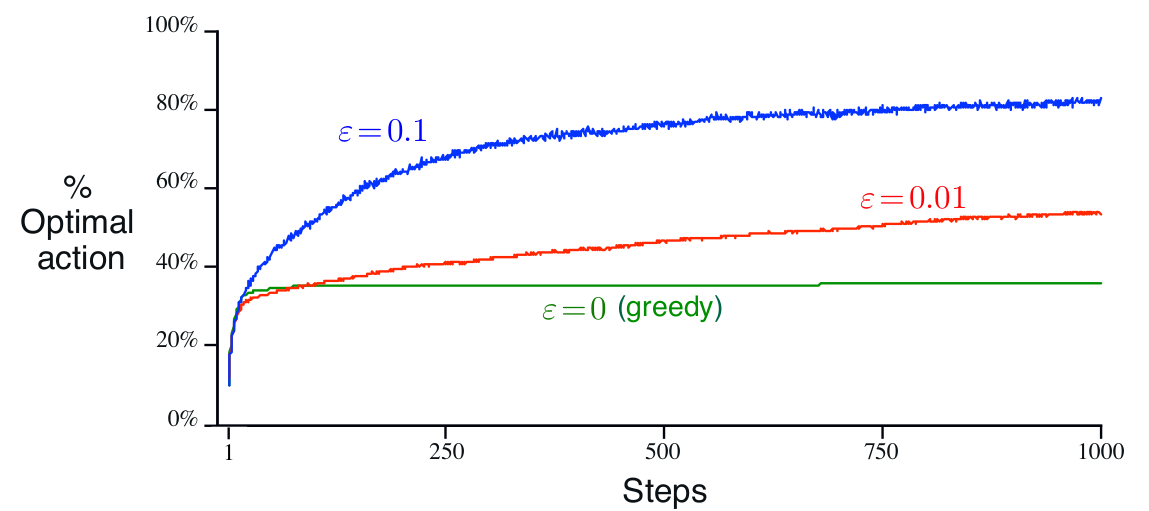
\includegraphics[scale=0.35]{images/eps_vs_optAction.png}
    \caption{Average performance of three agents using different $\epsilon$.  The data is averaged over 2000 runs.  Figure from \textit{Reinforcement Learning: An Introduction} by Sutton and Barto (2018).}
    \label{fig: eps_figure}
\end{figure}

During implementation, $\epsilon$ should decay out as $Q_t(a)$ approaches $q_*(a)$ to ensure knowledge of the agent is being adequately exploited. For non-stationary problems, $\epsilon > 0 \; \forall t$ to ensure other action values have not changed.

Algorithms to solve the \textit{k}-armed bandit problem are easily applied to situations where the concept of state is inert and only the actions are of concern;  a near impossibility in the real world.  

\subsubsection{Contextual Bandit}

A natural extension of the \textit{k}-armed bandit is associative search.  In associative search (sometimes called contextual bandit), different policies are associated with different situations \cite{bartosuttonbrouwer}.  Equation \ref{eq: state-action-value} is the extension of Equation \ref{eq:01value} in the associative search problem.

\begin{equation}
    \centering
    q_*(x, u) = \mathbb{E}[R_t | X_t = x, U_t = u]
    \label{eq: state-action-value}
\end{equation}

Associative search is known as the method between \textit{k}-armed bandits and reinforcement learning.  In associative search, the objective is to associate optimal policies to different situations, but only maximizing the \textit{immediate} reward.  Often times, near term sacrifices are required to initiate the trajectory to a large lump sum reward at the terminal state.  For example, heavy capital and time investment is required for University in the short term.  However, the long term gain is so great that it outweighs the short term losses, making going to University an optimal policy for many individuals.

In order to find the true optimal policy (i.e., policy that returns the greatest rewards over a long time period), the topic of reinforcement learning is developed.  In reinforcement learning, sequential decision making is explored to identify the delayed reward signals from different actions and to ultimately find the optimal policy, $\pi^*$.  